\documentclass{article}
\usepackage{amsfonts, amsthm, amsmath, amssymb, mathtools, ulem, mathrsfs, physics, esint, siunitx, tikz-cd}
\usepackage{pdfpages, fullpage, color, microtype, cancel, textcomp, markdown, hyperref, graphicx}
\usepackage{enumitem}
\graphicspath{{./images/}}
\usepackage[english]{babel}
\usepackage[autostyle, english=american]{csquotes}
\MakeOuterQuote{"}
\usepackage{xparse}
\usepackage{tikz}

% fonts
\def\mbb#1{\mathbb{#1}}
\def\mfk#1{\mathfrak{#1}}
\def\mbf#1{\mathbf{#1}}
\def\tbf#1{\textbf{#1}}

% common bold letters
\def\bP{\mbb{P}}
\def\bC{\mbb{C}}
\def\bH{\mbb{H}}
\def\bI{\mbb{I}}
\def\bR{\mbb{R}}
\def\bQ{\mbb{Q}}
\def\bZ{\mbb{Z}}
\def\bN{\mbb{N}}

% brackets
\newcommand{\br}[1]{\left(#1\right)}
\newcommand{\sbr}[1]{\left[#1\right]}
\newcommand{\brc}[1]{\left\{#1\right\}}
\newcommand{\lbr}[1]{\left\langle#1\right\rangle}

% matrices
\newcommand{\m}[2][b]{\begin{#1matrix}#2\end{#1matrix}}
\newcommand{\arr}[3][\sbr]{#1{\begin{array}{#2}#3\end{array}}}

% misc
\NewDocumentCommand{\app}{O{x} O{\infty}}{\xrightarrow{#1\to#2}}
\newcommand{\sse}{\subseteq}
\renewcommand{\ss}{\subset}
\newcommand{\vn}{\varnothing}
\newcommand{\e}{\epsilon}
\newcommand{\vp}{\varphi}
\renewcommand{\th}{\theta}
\newcommand{\inv}{^{-1}}
\newcommand{\imp}{\implies}
\newcommand{\impleft}{\reflectbox{$\implies$}}
\renewcommand{\ip}[2]{\lbr{#1,#2}}
\renewcommand{\bar}{\overline}
\DeclareMathOperator{\cis}{cis}
\DeclareMathOperator{\Arg}{Arg}
\renewcommand{\d}{\partial}
\newcommand{\pf}{\tbf{Proof. }}
\DeclareMathOperator{\fl}{fl}

% title
\title{Scientific Computing HW 1}
\author{Ryan Chen}
%\date{\today}
\setlength{\parindent}{0pt}


\begin{document}
	
\maketitle



\begin{enumerate}
	
	
	
	\item
	
	\begin{enumerate}
		
		
		
		\item The expressions result in equal floating point numbers since
		\begin{align*}
			\fl((x*y)+(z-w)) &= \fl((z-w))+(x*y) & \fl(a+b)=\fl(b+a) \\
			&= \fl((z-w)+(y*x)) & \fl(a*b)=\fl(b*a)
		\end{align*}
	
	
	
		\item Let $\e_1,\e_2,\e_3,\e_4$ be the relative error in computing $x+y,(x+y)+z,y+z,x+(y+z)$ respectively.
		\begin{align*}
			\fl((x+y)+z) &= ((x+y)(1+\e_1)+z)(1+\e_2) \\
			&= (x+y)(1+\e_1) + z + ((x+y)(1+\e_1)+z)\e_2 \\
			&= x + y + (x+y)\e_1 + z + (x+y+z)\e_2 + (x+y)\e_1\e_2 \\
			&= (x+y+z) + (x+y)\e_1 + (x+y+z)\e_2 + (x+y)\e_1\e_2
		\end{align*}
		Similarly,
		\[\fl(x+(y+z)) = \fl((y+z)+x) = (y+z+x) + (y+z)\e_3 + (y+z+x)\e_4 + (y+z)\e_3\e_4\]
		In general the expressions do not result in equal floating point numbers.
		
		
		
		\item Write $H$ for oneHalf. Floating point multiplication by 1/2 is always exact; to multiply a floating point number by 1/2, simply decrease the exponent by 1. In light of this, the exact result of $(x*H)+(y*H)$ equals the exact result of $x+y$ but with its exponent decreased by 1. In other words, the exact result of $(x*H)+(y*H)$ equals the exact result of $(x+y)*H$. Thus these expressions give equal floating point values.
		
		
		
		\item In general floating point multiplication by 1/3 is not exact, i.e. it produces relative errors. Write $T$ for oneThird. Let $\e_1,\e_2,\e_3,\e_4,\e_5$ be the relative errors of computing $x*T,y*T,(x*T)+(y*T),x+y,(x+y)*T$ respectively.
		\begin{align*}
			\fl((x*T)+(y*T)) &= ((xT)(1+\e_1)+(yT)(1+\e_2))(1+\e_3) \\
			&= \sbr{(x+y) + x\e_1 + y\e_2 + (x+x\e_1+y+y\e_2)\e_3}T \\
			&= \sbr{(x+y) + x(\e_1+\e_3) = y(\e_2+\e_3) + x\e_1\e_3 + y\e_2\e_3}T
		\end{align*}
		\begin{align*}
			\fl((x+y)*T) &= (x+y)(1+\e_4)T(1+\e_5) \\
			&= ((x+y)+(x+y)\e_4)(1+\e_5)T \\
			&= \sbr{(x+y) + x(\e_4+\e_5) + y(\e_4+\e_5) + (x+y)\e_4\e_5}T
		\end{align*}
		In general the expressions do not result in equal floating point numbers.
		
		
	\end{enumerate}
	
	
	
	\item We state some preliminaries for this problem. Let $f^n$ denote the $n-$fold composition of $f$. Define the left bit shift map
	\[g:[0,1]\to[0,1],
	\quad g(x) =
	\begin{cases}
		2x, & x<\frac12 \\
		2x-1, & x\ge\frac12
	\end{cases}\]
	The name of the map comes from the fact that, for binary expansions of numbers in $[0,1]$,
	\[g(0.b_1b_2\dots) = 0.b_2b_3\dots,
	\quad b_i\in\brc{0,1}\]
	
	
	We also state some lemmas.
	
	
	\tbf{Lemma 1.} $f\circ g=f^2$.
	
	\pf Split into cases.
	\begin{itemize}
		\item If $0\le x<\frac14$ then $0\le 2x<\frac12$, so
		\[f(g(x)) = f(2x) = 4x\]
		\[f(f(x)) = f(2x) = 4x\]
		\item If $\frac14\le x<\frac12$ then $\frac12\le 2x<1$, so
		\[f(g(x)) = f(2x) = 2-4x\]
		\[f(f(x)) = f(2x) = 2-4x\]
		\item If $\frac12\le x<\frac34$ then $0\le 2x-1<\frac12$ and $\frac12<2-2x\le1$, so
		\[f(g(x)) = f(2x-1) = 4x-2\]
		\[f(f(x)) = f(2-2x) = 4x-2\]
		\item If $\frac34\le x\le 1$ then $\frac12\le 2x-1\le 1$ and $0\le 2-2x\le\frac12$, so
		\[f(g(x)) = f(2x-1) = 4-4x\]
		\[f(f(x)) = f(2-2x) = 4-4x\]
	\end{itemize}
	
	
	\tbf{Lemma 2.} $f\circ g^n = f^{n+1}$ for all $n\ge1$.
	
	\pf Repeatedly apply lemma 1.
	\[f\circ g^n = f\circ\underbrace{g\circ\dots\circ g}_{n\text{ times}}
	= f^2\circ\underbrace{g\circ\dots\circ g}_{n-1\text{ times}}
	= \dots
	= f^{n+1}\]
	
	
	\tbf{Lemma 3.} The sequence $f^n(x_0)$ (in $n$) is eventually $p-$periodic iff there exists $N$ such that $f^{N+p}(x_0)=f^N(x_0)$.
	
	\pf $(\imp)$ Eventual periodicity gives $N$ such that $f^{n+p}(x_0)=f^n(x_0)$ for all $n\ge N$. In particular $f^{N+p}(x_0)=f^N(x_0)$.
	
	$(\impleft)$ Let $p=M-N$. Then for all $n\ge N$,
	\[f^{n+p}(x_0) = f^{n-N+N+p}(x_0)
	= f^{n-N}(f^{N+p}(x_0))
	= f^{n-N}(f^N(x_0))
	= f^n(x_0)\]
	Thus the sequence $f^n(x_0)$ is eventually $p-$periodic.
	
	
	The last lemma is taken for granted since it is a relatively well--known fact.
	
	\tbf{Lemma 4.} A number is rational iff it has an eventually periodic binary expansion.
	
	
	\begin{enumerate}
		
		
		
		\item We find fixed points in the interval $[0,1/2)$ by
		\[x^* = f(x^*)
		\imp x^* = 2x^*
		\imp x^* = 0\]
		We find fixed points in the interval $[1/2,1]$ by
		\[x^* = f(x^*)
		\imp x^* = 2 - 2x^*
		\imp x^* = \frac23\]
		Thus the fixed points are $x^*=0,2/3$.
		
		
		
		\item Fix $x_0\in\bQ\cap[0,1]$. By lemma 4, $x_0/2\in\bQ$ admits an eventually periodic binary expansion. Using the left bit shift map $g$, the sequence $g^n(x_0/2)$ is eventually periodic, say with period $p$, so lemma 3 gives $N$ such that $g^{N+p}(x_0/2)=g^N(x_0/2)$. Note that $f(x_0/2)=x_0$ since $0\le x_0/2\le1/2$. Then
		\begin{align*}
			f^{N+p}(x_0) &= f^{N+p+1}\br{\frac{x_0}{2}} & f\br{\frac{x_0}{2}}=x_0 \\
			&= f\br{g^{N+p}\br{\frac{x_0}{2}}} & \text{by lemma 2} \\
			&= f\br{g^N\br{\frac{x_0}{2}}} & g^{N+p}(x_0/2)=g^N(x_0/2) \\
			&= f^{N+1}\br{\frac{x_0}{2}} & \text{by lemma 2} \\
			&= f^N(x_0) & f\br{\frac{x_0}{2}}=x_0
		\end{align*}
		Thus by lemma 3, the sequence $f^n(x_0)$ is eventually $p-$periodic.
		
		
		
		\item Fix a period $p$. Referring to the argument in the last part, it suffices to find $x_0\in\bQ\cap[0,1]$ such that $g^{N+p}(x_0/2)=g^N(x_0/2)$, so that the sequence $f^n(x_0)$ is eventually $p-$periodic.
		
		Write a binary expansion of $x_0\in[0,1]$,
		\[x_0 = 0.b_1b_2\dots,
		\quad b_i\in\brc{0,1}\]
		Imposing the condition $g^{N+p}(x_0/2)=g^N$ for some $N$ gives
		\[0.b_{N+p}b_{N+p+1}\dots = 0.b_Nb_{N+1}\dots\]
		which is equivalent to $b_{n+p}=b_n$ for all $n\ge N$. Plugging into the expansion,
		\[x_0 = 0.b_1b_2\dots b_{N-1}\bar{b_Nb_{N+1}\dots b_{N+p-1}}\]
		This is an eventually periodic expansion, so by lemma 4, $x_0\in\bQ\cap[0,1]$.
		
		In conclusion, given $p$, the sequence $f^n(x_0)$ is eventually $p-$periodic for $x_0$ with binary expansion
		\[x_0 = 0.b_1b_2\dots b_{N-1}\bar{b_Nb_{N+1}\dots b_{N+p-1}}\in\bQ\cap[0,1],
		\quad N\ge1,
		\quad b_i\in\brc{0,1},
		\quad 1\le i\le N+p-1\]
		
		
		
		
		\item Below are a few sequences of iterates.
		
		\begin{center}
			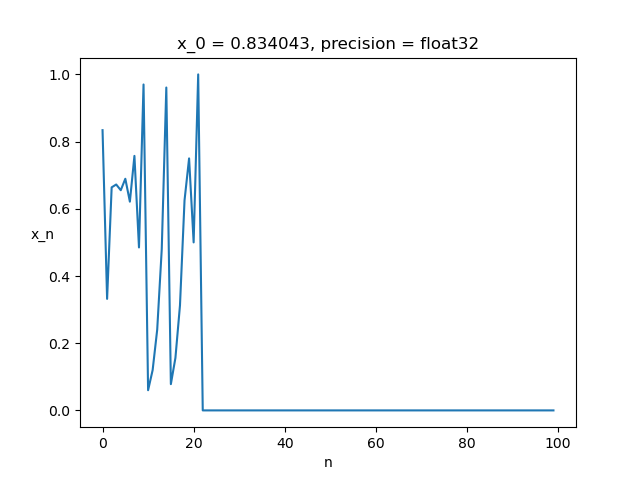
\includegraphics[scale=.4]{hw1 run = 0, precision = float32}
			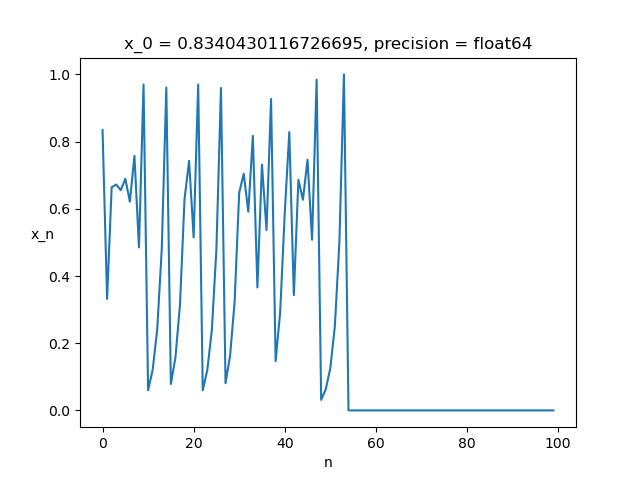
\includegraphics[scale=.4]{hw1 run = 0, precision = float64}
			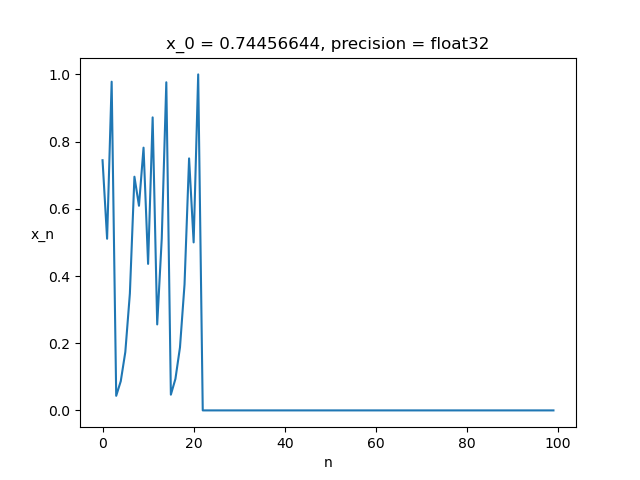
\includegraphics[scale=.4]{hw1 run = 1, precision = float32}
			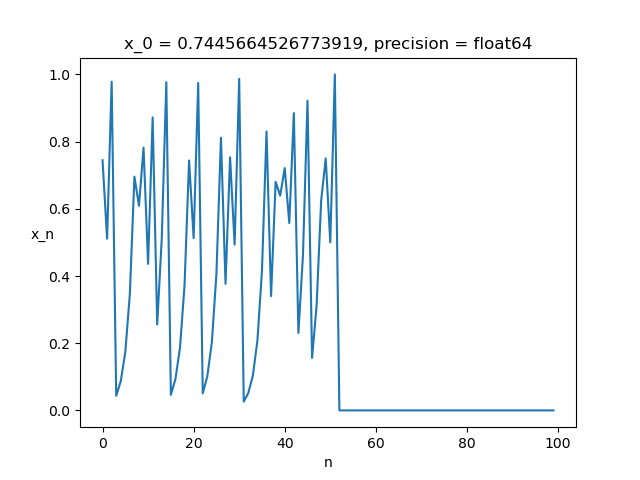
\includegraphics[scale=.4]{hw1 run = 1, precision = float64}
			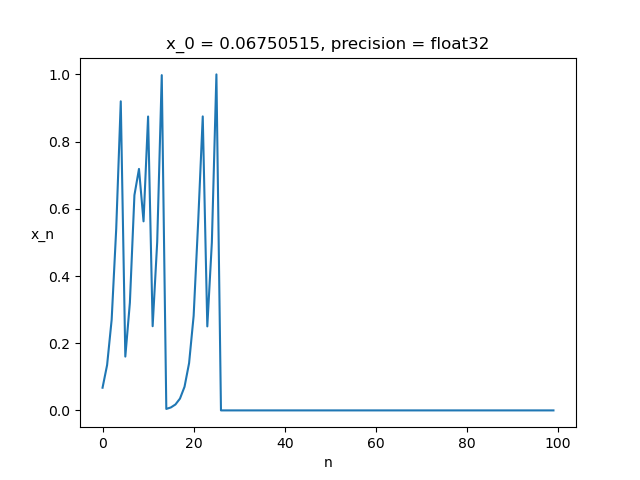
\includegraphics[scale=.4]{hw1 run = 2, precision = float32}
			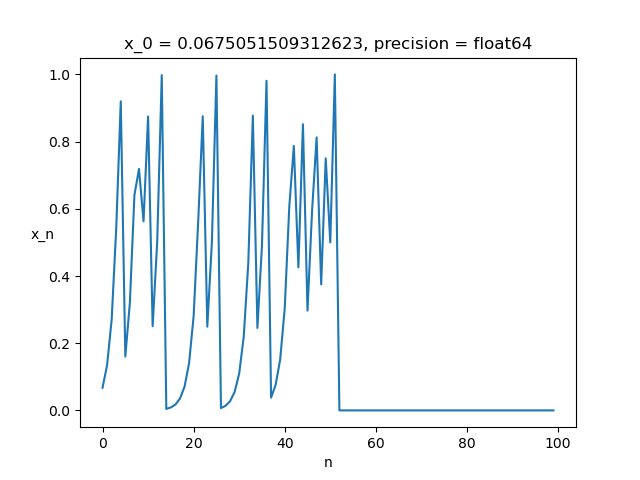
\includegraphics[scale=.4]{hw1 run = 2, precision = float64}
			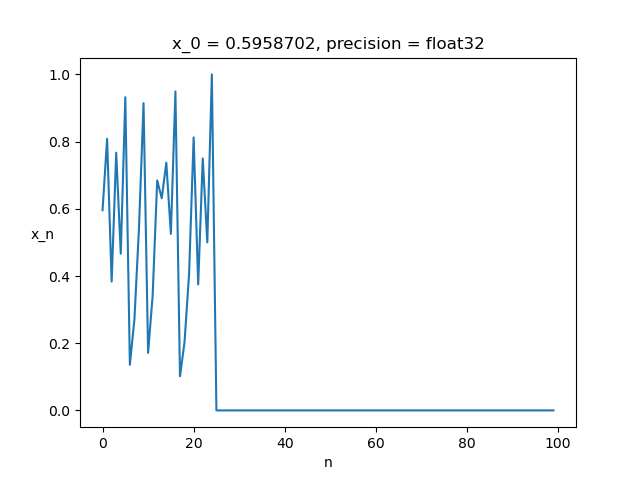
\includegraphics[scale=.4]{hw1 run = 3, precision = float32}
			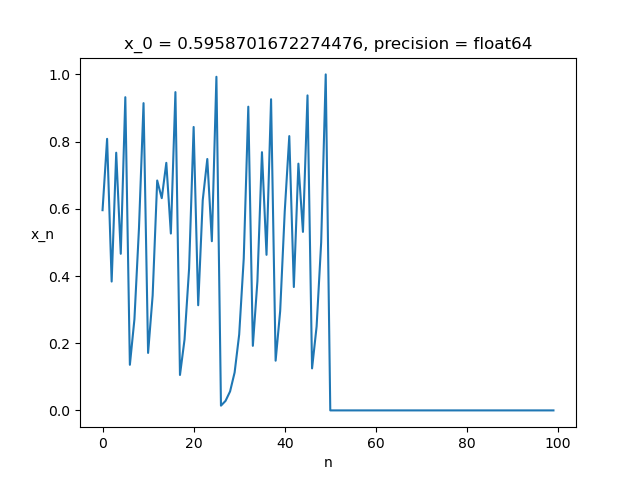
\includegraphics[scale=.4]{hw1 run = 3, precision = float64}
		\end{center}
	
		The iterates eventually become zero, and this happens even faster for single precision.
		
		
		\item Floating point numbers have terminating binary expansions, so iteration under the left bit shift map $g$ eventually vanishes. This, along with the facts that $f^{n+1}=f\circ g^n$ (lemma 2) and $f(0)=g(0)=0$, implies that iteration of floating point numbers under $f$ eventually vanishes. Moreover, single precision floating point numbers have fewer binary digits, which is why iteration under $f$ vanishes faster than for double precision.
		
		
	\end{enumerate}
	
	
	
\end{enumerate}
	
	
\end{document}